\documentclass{article} % For LaTeX2e
\usepackage{nips13submit_e,times}
\usepackage{hyperref}
\usepackage{url}
\usepackage{graphicx}
\usepackage{tikz}
\usepackage{pgfplots}
\usepackage{subcaption}
\usepackage{amsfonts, amsmath}
%\documentstyle[nips13submit_09,times,art10]{article} % For LaTeX 2.09

\DeclareMathOperator{\corr}{corr}

\title{Unsupervised Feature Learning for Object Classification}


\author{
  Laxman Dhulipala, Harry Gifford, Wangzi He \\
  Department of Computer Science\\
  Carnegie Mellon University University\\
  Pittsburgh, PA 15213 \\
  \texttt{\{ldhulipa, hgifford, wangzih\}@andrew.cmu.edu} \\
}

% The \author macro works with any number of authors. There are two commands
% used to separate the names and addresses of multiple authors: \And and \AND.
%
% Using \And between authors leaves it to \LaTeX{} to determine where to break
% the lines. Using \AND forces a linebreak at that point. So, if \LaTeX{}
% puts 3 of 4 authors names on the first line, and the last on the second
% line, try using \AND instead of \And before the third author name.

\newcommand{\fix}{\marginpar{FIX}}
\newcommand{\new}{\marginpar{NEW}}

\nipsfinalcopy % Uncomment for camera-ready version

\begin{document}

\maketitle

\begin{abstract}
  A major theme in modern object recognition research has been the use of
  features to boost classification techniques. Stemming from the seminal work
  of Viola and Jones, features and feature learning techniques have been used
  year after year to improve existing object recognition algorithms, and increase
  classification rates. In this work, we implement and evaluate an object classification framework
  that first learns a dictionary of features, and subsequently uses this feature basis
  to represent and classify images into categories. We evaluate our classification framework
  by analyzing its performance on the CIFAR-10 dataset, and also consider several optimizations
  and heuristics to help boost performance.
\end{abstract}

\section{Introduction}

Object Recognition as a field has its roots firmly embedded in a long history
of research in Neuroscience. Stemming from Hubel and Wiesel's discovery in the
late 1950's of complex and simple cells, researchers have been captivated by using
techniques and ideas from neuroscience as building blocks for robust object
classification in a machine\cite{hubel}. To this end, ideas from neuroscience such as the Perceptron
algorithm, convolution neural networks and most recently, deep belief networks have all
had tremendous success in object recognition and machine learning.

A fundamental step for many object recognition algorithms is to learn hierarchies
of features from images. Learnt features from a dataset afford the algorithm designer
to then represent images in the dataset as linear combinations of the learnt features.
In some sense, this is the most natural reason to learn features, as they allow one
to transform the space of images into the space of images as represented by their features.
This transformed space typically produces better results when running object classification
algorithms - even naive classification techniques such as $k$-nearest neighbors.

Feature heirarchies can be learnt in a variety of ways, from semi-supervised learning
algorithms to fully unsupervised learning algorithms.
Our approach to feature learning relies on an elegant and simple algorithm that was
recently published by Adam Coates and Andrew Ng \cite{coates11}. They propose the use
of $k$-means clustering for feature learning as it is a simple and easily paralellizable
algorithm that can be deployed at scale. In an earlier work, they show how $k$-means in
practice is highly competitive against the state-of-the-art feature learning algorithms,
often beating them. In particular, they show a surprising result that
$k$-means based feature learning with a single layer neural network achieves state-of-the-art
error rate on the CIFAR-10 dataset.

\section{Related Work}

Object classification has had a long history of research and experimental results. In
particular, many researchers in the past decade have made attempts at understanding the
CIFAR-10 dataset with varying degrees of success. In this section we first describe
several other methods for performing feature learning, consider several algorithms which
use features to boost object classification performance, and finally describe the success
of some of these methods on the CIFAR-10 dataset.

Feature learning can be split into three categories - supervised approaches
semi-supervised approaches, and lastly unsupervised feature learning.
In terms of semi-supervised approaches, perhaps the most classic approach is that of
Nigam et al. who describes how to
learn text classifiers when there are limited number of labeled examples \cite{nigam}.
They in a sense
overcome the dearth of labeled examples by using unlabeled documents to support the data.
This is a somewhat counterintuitive result, but can be rationalized by understanding that
unlabeled data, based on inferences about which class an unlabeled example belongs to can
be used to boost the joint probability distribution of features in the document. The authors
ultimately used EM (Expectation Maximization) with the assumption that the underlying data
arises from a mixture model to classify text.

Another recent feature learning approach is pioneered by Raina et al. and runs under the
moniker of Self-Taught Learning \cite{raina}. Self-Taught Learning works similarly to
the EM-based
approach described above, but makes no assumptions about the underlying distribution or
classes of the unsupervised data (there is no assumption that the unlabeled data even
contains objects that are provided in the training and test datasets). Instead, they exploit
the fact that the unsupervised data is a collection of natural images. This makes their
algorithm significantly easier to apply in practice, as one can simply take a set of labeled
examples, and augment it with an enormous unlabeled data-set of support examples.

Both approaches are interesting due to their real world practicality - which we are deeply
concerned with. Both approaches augment their small set of labeled examples with a large
number of unlabeled examples, and use the unlabeled examples to improve performance on the
test dataset. In the world, labeled examples are prohibitively costly -
therefore it is imperative to have techniques that will be almost fully unsupervised.

\section{Datasets}
We choose to evaluate our object classification algorithm on the CIFAR-10 dataset. CIFAR-10 is a standard dataset of 32x32 color images of a single object in one of ten categories. It contains 60,000 labeled images, with 50,000 for training and 10,000 for testing.

\begin{figure}
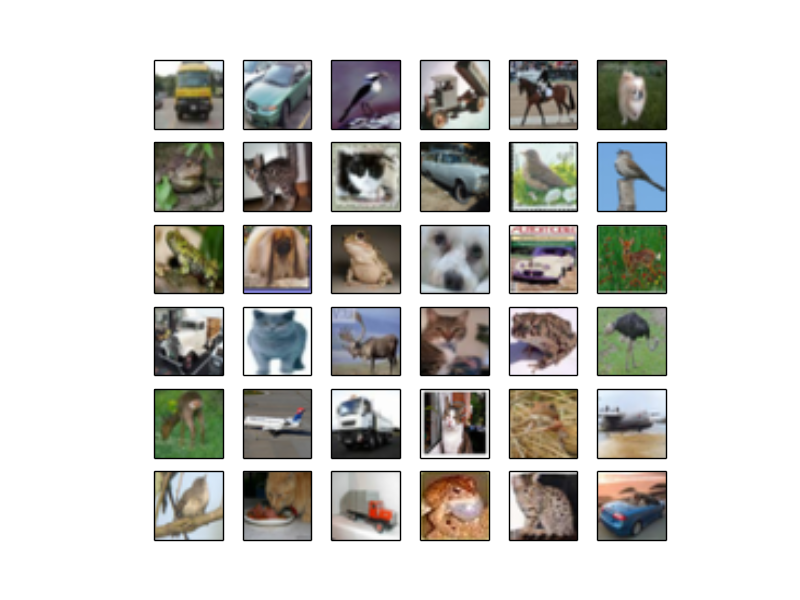
\includegraphics[width=0.5\columnwidth]{./images/examples.png}
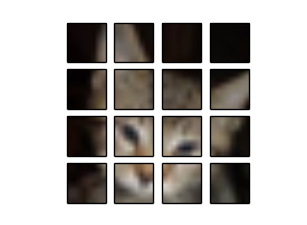
\includegraphics[width=0.5\columnwidth]{./images/extracted_patches.png}
\caption{Example images from the CIFAR-10 dataset, and a dicing of one particular image into 16 $8 \times 8$ non-overlapping patches. Normally, we will infact allow patches to overlap in order to support translation invariance.}
\end{figure}

\section{Algorithm}
We now describe the image classification algorithm, based on \cite{coates11}. Assume that we have a dataset with large amounts of unlabeled data from a similar domain to the classification algorithm. Notice that this assumption differs from that in semi-supervised learning in that we are not garanteed that the unlabeled data contains only examples from what we want to classify. For example, if we are classifying birds vs. planes we may have images of buildings or plants in the unlabeled data.

\begin{figure}
  \centering
  \begin{subfigure}[h]{0.45\columnwidth}
    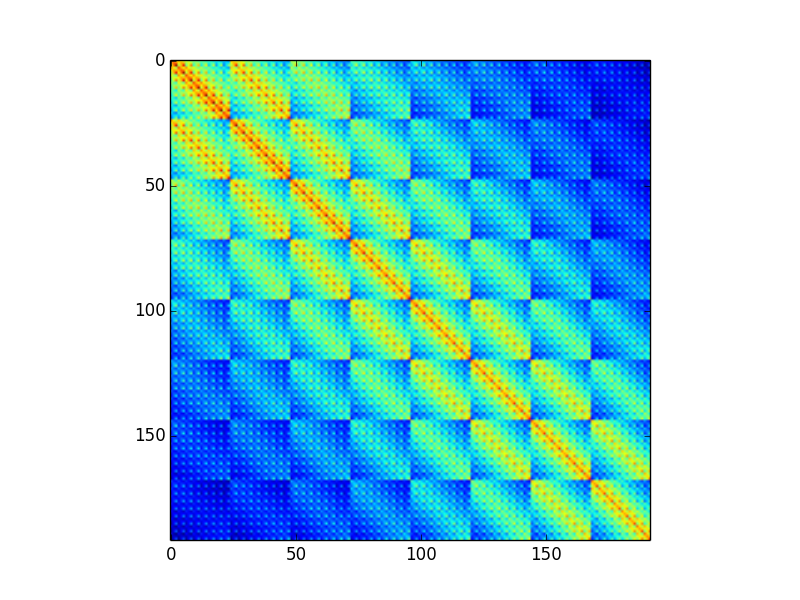
\includegraphics[width=\columnwidth]{./images/before_whiten.png}
    \caption{Before whitening}
    \label{figBefore}
  \end{subfigure}
  \hspace{0.04\columnwidth}
  \centering
  \begin{subfigure}[h]{0.45\columnwidth}
    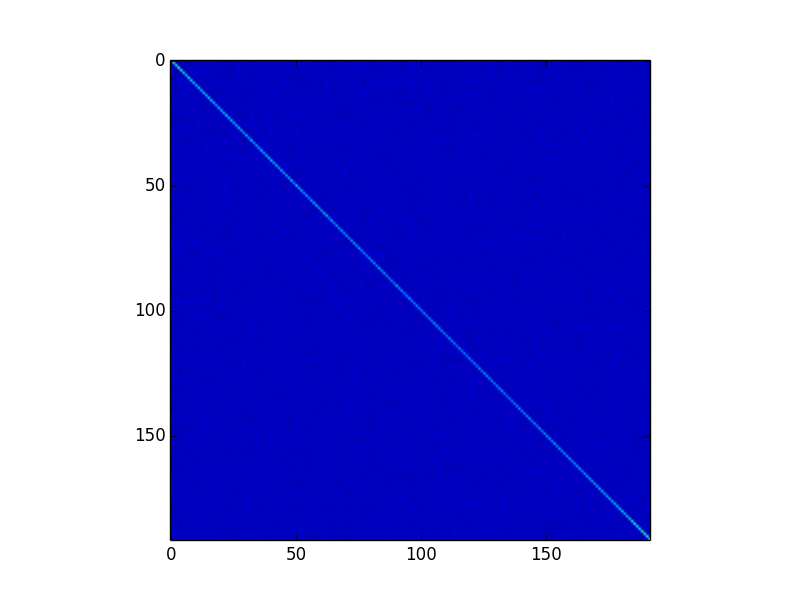
\includegraphics[width=\columnwidth]{./images/after_whiten.png}
    \caption{After whitening}
    \label{figAfter}
  \end{subfigure}
  \caption{Covariance matrix of image patches before and after whitening (red means large value, blue means small value). As can be seen from \ref{figBefore} there is a large amount of correlation between neighboring pixels, which we seek to remove.}
  \label{whitening}
\end{figure}

\begin{enumerate}
\item Extract random patches from the unsupervised data. Standardize the patches, so that each patch has mean 0 and standard deviation 1. Whiten the input patches to make the covariance matrix of the each patch approximately the identity matrix. This can be done via PCA or ZCA, as described in \cite{kriz}. The effect of whitening on the can be seen in Figure~\ref{whitening}.

  This means that we do not waste learning resources learning unneccessary imformation, such as knowing that neighboring pixels are more likely to have similar colors.
  In Figure \ref{figEigenvectors} we show the eigenvectors we extract when performing PCA/ZCA. We see that each eigenvector corresponds to a different frequency basis. These eigenvectors are very similar to those from the discrete cosine transform (DCT), which is often used in image compression.

  We can also optionally use PCA to reduce the dimensionality of the data. This doesn’t help with accuracy of the quality of features learned, but it does speed up the pipeline significantly. In fact, we show in the analysis section that performing PCA is not a good idea in general.

\item Cluster these patches using K-means with the euclidean or cosine distance metric. Generally it is best to pick as large a k as the amount of data will allow, however metrics such as silhouette scoring etc. can also be useful if data is severely limited. Figure \ref{fig_centroids} shows the centroids learned when performing euclidean K-means with 100 centroids. These features are similar to those learned by blind source seperation, such as ICA \cite{hoyer}

\item For each training example, extract all patches from each image. Normalize and whiten these patches as in 1. Get some measure of ‘distance’ from the centroids learned by K- means. There are many approaches that can be taken here. For example, we can find the euclidean distance to each patch or convolve each centroid with the whitened patches from the image. We can also use the distance metric suggested by Coates which has the benefit of adding some sparsity: $f_{ij} = \max(0, \mu_i - x_{ij}$), where $\mu_i$ is the average distance from the patch to each centroid and $x_{ij}$ is the distance from patch i to centroid j.

\item Pool these feature responses in order to reduce the dimensionality. One approach is to pool the responses into a $n \times n$ grid.

\item Pass these features into your favorite linear classifier (e.g. SVM or logistic regression) or pass these features back into the K-means pipeline described above. If we reuse the k means pipeline, it is important to develop some way to reduce the dimensionality of the features in higher levels of the pipeline. One way we can do this is to measure the correlation in terms of activation between different features, and then combine the highly correlated features. For example, this can happen with edges that share very similar angles, but perhaps have a slighly different translations.

  We also experimented with using sparse k means as described in \cite{tibs10} in the higher layers, which helps to filter out those features that do not significantly help representation.
\end{enumerate}

\begin{figure}
  \centering
  \begin{subfigure}[h]{0.45\columnwidth}
    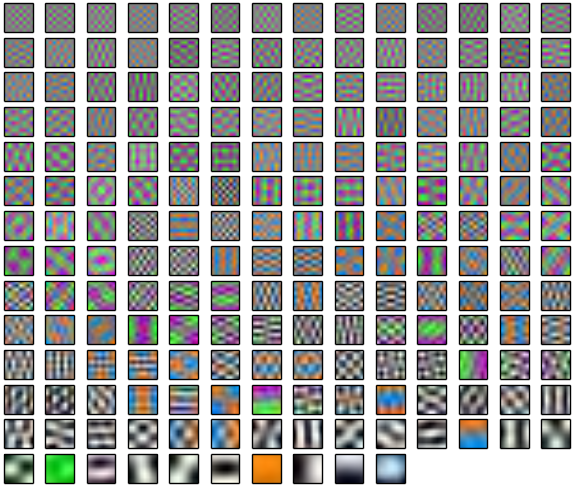
\includegraphics[width=\columnwidth]{./images/eigs192.png}
    \caption{All 192 eigenvectors of a selection of 8x8 color patches from the CIFAR dataset.}
    \label{figEigenvectors}
  \end{subfigure}
  \hspace{0.04\columnwidth}
  \centering
  \begin{subfigure}[h]{0.45\columnwidth}
    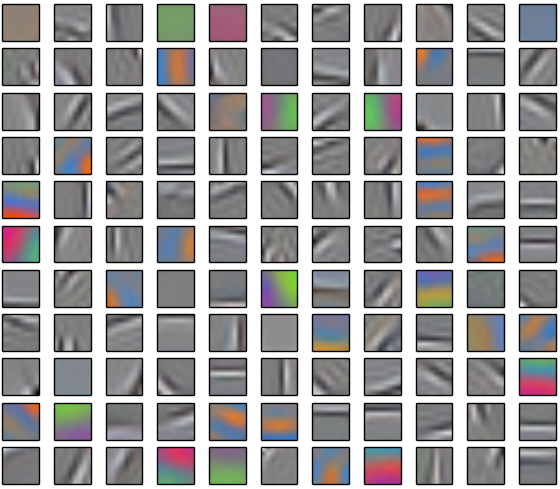
\includegraphics[width=\columnwidth]{./images/patches100.png}
    \caption{100 centroids learned from applying K-means to 8x8 patches extracted from natural images. Notice the similarity to Gabor wavelets.}
    \label{fig_centroids}
  \end{subfigure}
\end{figure}

\subsection{Deeper layers}

One of the benefits of feature learning is that we can extend our learner to take the output features from one layer of the k-means learner and use them as input to the next layer. We have to be careful when extending the feature learner to multiple layers, since we can end up with very high dimensional features. Therefore we have to perform some kind of feature selection. There are two main ways to do this, construct many local receptive fields based on some kind of similarity or correlation metric, or to perform feature selection within a regularized form of k-means.

\subsubsection{Fusing Features}

We can use the idea of the receptive field \cite{barrow87} to select a small subset of highly related features with which we will pass into the usual feature learning pipeline described above.

\cite{coates} have suggested using the squared correlation between two features as a measure of their dependency. The dependency metric is

\begin{equation}
d(z_j, z_k) = \corr(z_j^2, z_k^2) = \mathbb{E}[z_j^2z_k^2-1]/\sqrt{\mathbb{E}[z_j^4 - 1]\mathbb{E}[z_k^4-1]}
\end{equation}

We then select the top $R$ features (100 or so) from one random seed feature. We then solely use these top $R$ features to learn a higher level set of features. We then combine this with the features learned from other seeds and these become our new features.

\subsubsection{Regularized k-means}

\begin{figure}
  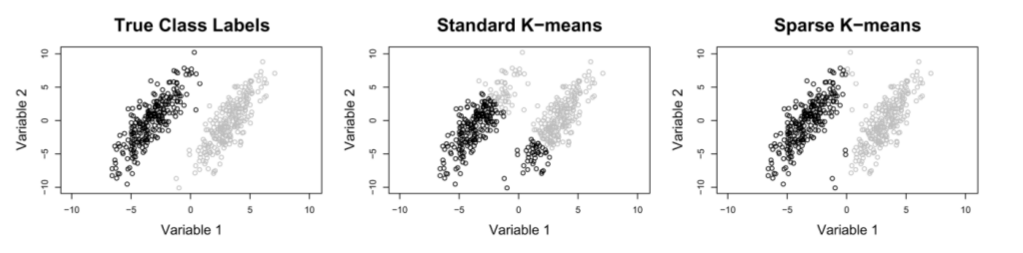
\includegraphics[width=\columnwidth]{./images/sparse.png}
  \caption{Sparse K-means helps us perform feature selection. Notice that without it, k-means gets distracted by the irrelevant features.}
  \label{figSparseKM}
\end{figure}

K-means is not by default robust to non-discriminative features. Specifically, if we have a lot of features that will not help us to seperate different classes, then those features will actually hurt the clustering algorithm. This can happen often when we have high dimensional data, i.e. $p \gg n$. This problem is shown in Figure~\ref{figSparseKM}. Here, we notice that the second feature does not help us to determine which class a point belongs to. Worse, in this case it actually changes the assignment of the clusters. We want to remove these features from consideration.

Here is where we can use a regularized form of k-means, which assigns a weight to each feature as it clusters.

Specifically, we wish to maximize the weighted between cluster sum of squares, which is simply framed as

\begin{equation}
\begin{aligned}
& \underset{x}{\text{maximize}}
& & \sum_{j=1}^p w_j\left(\frac{1}{n}\sum_{i=1}^n\sum_{i'=1}^nd_{i, i', j}-\sum_{k=1}^K \frac{1}{n_k}\sum_{i, i'\in C_k} d_{i, i', j}\right) \\
& \text{subject to}
& & ||w||^2 \leq 1, \; ||w||_1\leq s, \; w \geq \mathbf{0}
\end{aligned}
\end{equation}

The $||w||_1 \leq s$ constraint ensures sparsity when $s$ is small. The $||w||^2 \leq 1$ constraint ensures that we have more than one non-zero feature.

The details of how we actually optimize this function are not important for our purposes, but the details are discussed at length in \cite{tibs10}, along with good methods for selecting $s$. We did not explore how $s$ changes the clustering results.

We can combine this method with the correlation idea above, which helps us to automatically throw out certain dimensions, which further reduces dimensionality.

\section{Experiments}

We analysed the above algorithm by implementing the full pipeline, and then testing the effects of changing certain parts. We will discuss the effect of depth, the effect of PCA for dimensionality reduction and the effect of sparse k-means.

\begin{table}
  \label{tableacc}
  \centering
  \begin{tabular}{|c|c|}
    \hline
    \textbf{Method} & \textbf{Accuracy}\\
    \hline
    Random & 10.0\%\\
    Raw pixels & 37.3\%\\
    K-means + all PCs & 77.9\%\\
    K-means + 0.99 variance & 50.0\%\\
    3 layers & 82.0\%\\
    Sparse 3 layers & 83.5\%\\
    \hline
  \end{tabular}
  \caption{Performance of the different methods we tried.}
\end{table}

Table~\ref{tableacc} shows the accuracy of different algorithms with all 50000 training examples from CIFAR-10. The algorithms were

\begin{itemize}
\item[1.] randomly choosing a class.
\item[2.] Taking the raw pixels from each image and feeding them into an SVM
\item[3.] Single layer K-means we have described above.
\item[4.] K-means with PCA run on the patches, keeping 99\% of the variance.
\item[5.] Stacking the K-means feature learner into a deep network.
\item[6.] 3-layer network, but we use sparse K-means at the deeper levels.
\end{itemize}

Since we have 10 classes in the dataset we tested, we want to do better than 10\% in classification. In fact, we really have a stricter baseline, since we have no interest in the classifier that the learned features are output. Therefore, we hope that our learned features will do better than raw pixels when fed into an off the shelf classifier, such as a linear SVM. In fact, as can be seen from Table~\ref{tableacc}, running an SVM against raw pixels performs poorly, suggesting that raw pixels do not make for a good feature representation for image classification. In fact, we suspect that most of the accuracy for this method is explained by the color of different images, since different classes have different distributions of color.

Running PCA on image patches also sacrifices a large amount of accuracy. If we were to run PCA on the data in Figure \ref{figSparseKM} we would not be able to get good clusters on the new space. This is reflected in the accuracy drop from using PCA based on the total variance of the data.

\subsection{PCA}

\begin{figure}
  \centering
  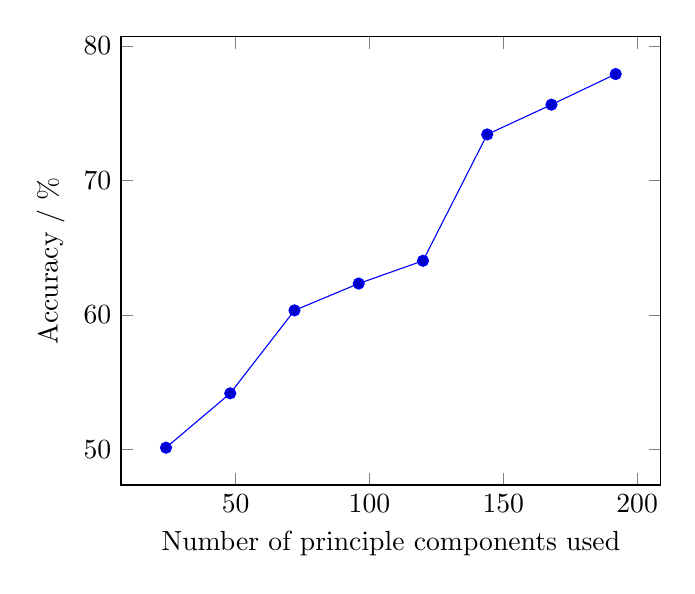
\begin{tikzpicture}
    \begin{axis}[
        xlabel={Number of principle components used},
        ylabel={Accuracy / \%}]
      ]
        \addplot coordinates {
          (24, 50.14)
          (48, 54.177)
          (72, 60.341)
          (96, 62.334)
          (120, 64.027)
          (144, 73.415)
          (168, 75.628)
          (192, 77.9)
        };
    \end{axis}
  \end{tikzpicture}
  \caption{Using PCA to perform dimension reduction is not always a good idea. }
  \label{graphPCA}
\end{figure}

We experimented with running principle component analysis (PCA) on the original image patches in order to reduce the dimensionality of the data before passing them into k-means. There are two benefits to reducing dimensionality before running k-means. The first is that with lower dimensions significantly less data is required for PCA to perform well. Secondly clustering in a low dimensional space takes up much less time and memory.

When we run PCA on the input image patches, we get a significant reduction in accuracy, as can be seen in Figure~\ref{graphPCA}. In fact, this reduction in accuracy makes a lot of sense, since we expect that most of the pixels in each patch will have a reasonably similar importance in representing each image, since the patches are extracted at random from the image.

We therefore suggest not running PCA (or any linear dimensionality reduction tool) on the data as a preprocessing step.

\bibliographystyle{acm}
\bibliography{ref}



\end{document}
